\subsection{Geometria}
\label{sec:teogeom}

\begin{figure}
	\center
	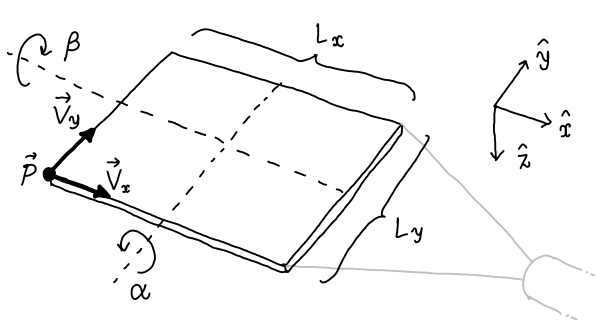
\includegraphics[width=25em]{geometriadef}
	\caption{\label{fig:geometriadef}
	Definizione del modello geometrico.
	Gli angoli $\alpha$ e $\beta$ sono nulli
	quando il lato della lastra ortogonale al loro asse di rotazione è orizzontale.
	Gli assi di rotazione sono riferiti alla lastra.}
\end{figure}

Esponiamo la modellizzazione geometrica dell'apparato ai fini di calcoli e simulazioni
(vedi \autoref{fig:geometriadef}).
Consideriamo ogni lastra di scintillatore come un parallepipedo.
Teniamo conto dei \emph{disallineamenti} cioè della posizione arbitraria nello spazio delle lastre,
supponendo però che sia poco diversa da quella ideale di lastre orizzontali, rettangolari e allineate verticalmente.
Chiamiamo $x$ la direzione orizzontale parallela ai tubi fotomoltiplicatori,
$y$ quella ortogonale,
$z$ la direzione verticale.
Assumiamo che la direzione verticale data dalla gravità
coincida con la media dei versori normali alle lastre.

Una lastra è descritta da un'\emph{origine} $\vec P$,
da due \emph{generatori} $\hat V_x$ e $\hat V_y$
e dalle lunghezze dei lati $L_x$ e $L_y$.
La superficie superiore della lastra è un parallelogramma descritto parametricamente da
\marginpar{Mettere il simbolo di versore anche nella figura.}
\begin{equation}
	\label{eq:lastra}
	\vec r(t_x, t_y) = \vec P + t_x L_x \hat V_x + t_y L_y \hat V_y,
	\quad t_x,t_y \in (0,1).
\end{equation}

\subsection{Raggi cosmici}

Poniamo che le traiettorie dei raggi cosmici siano rettilinee.
Per la seguente discussione trascuriamo lo spessore delle lastre.

\paragraph{Raggi}

Consideriamo una distribuzione di \emph{raggi}.
Un raggio è definito dalle variabili:
\begin{equation}
	\label{eq:raggio}
	\begin{array}{ll}
		t_x, t_y & \text{uniformi in $(0,1)$}, \\
		\phi     & \text{uniforme in $(0,2\pi)$}, \\
		u        & \text{distribuzione non fissata in $(0,1)$}.
	\end{array}
\end{equation}
Scegliamo una certa lastra che chiamiamo \emph{pivot}.
Da un raggio otteniamo una retta nello spazio parametrizzata come
\begin{align*}
	\vec r(t) &= \vec p + t \hat v, \quad \text{dove} \\
	\vec p    &= \vec r_\text{pivot}(t_x, t_y), \\
	\hat v    &= \sin\theta\cos\phi\,\hat x + \sin\theta\sin\phi\,\hat y + \cos\theta\,\hat z, \\
	\theta    &= \arccos u,
\end{align*}
e $\vec r_\text{pivot}$ è la parametrizzazione del pivot secondo la \eqref{eq:lastra}.

\paragraph{Accettanza}

Un'\emph{accettanza} è la probabilità che un raggio
faccia scattare alcune lastre (lastre in \emph{coincidenza})
e non altre (lastre in \emph{anticoincidenza}).
Richiediamo che il pivot sia sempre in coincidenza.
Ogni lastra ha un'\emph{efficienza},
cioè la probabilità che un raggio che passa per la lastra la faccia scattare.
Sia $\epsilon(L)$ l'efficienza della lastra $L$.
Sia
\begin{equation*}
	w_r(L) = \begin{cases}
		1 & \text{se il raggio $r$ passa per la lastra $L$,} \\
		0 & \text{se non passa,}
	\end{cases}
\end{equation*}
dove $r$ sono le variabili della \eqref{eq:raggio}.
Allora l'accettanza è
\begin{equation}
	\label{eq:acc}
	Q = \int p(r) \mathrm{d} r
	\left( \prod_\text{$L$ in coinc.} w_r(L) \epsilon(L) \right)
	\cdot \left( \prod_\text{$L$ in anticoinc.} \big(1 - w_r(L) \epsilon(L)\big) \right).
\end{equation}

\paragraph{Flusso totale}

Consideriamo una distribuzione non normalizzata di raggi su tutto il \emph{piano orizzontale} $(x,y)$,
cioè sostituiamo le variabili $t_x$, $t_y$ della \eqref{eq:raggio} con $x$, $y$.
Sia il \emph{flusso totale $\Phi$} la densità di raggi per unità di area orizzontale,
cioè integriamo le variabili $\phi$ e $u$.
Chiamiamo \emph{espressione logica} una specificazione di quali lastre sono in (anti)coincidenza.
Poiché abbiamo richiesto che il pivot sia in coincidenza,
usare la distribuzione dei raggi su tutto il piano orizzontale è equivalente
a usare la distribuzione solo sulla superficie del pivot.
Per passare da una distribuzione all'altra,
il jacobiano non è altro che la proiezione sul piano orizzontale dell'area del pivot
\begin{equation*}
	A_\text{hor} = L_x \sqrt{1-(\hat V_x\hat z)^2} \cdot L_y \sqrt{1-(\hat V_y\hat z)^2},
\end{equation*}
dove i simboli hanno lo stesso significato che nella \eqref{eq:lastra}
e sono riferiti al pivot.
Sia il \emph{rate $R$} di un'espressione logica l'analogo dell'accettanza
ma con la distribuzione di raggi non normalizzata sul piano orizzontale\footnote{Non abbiamo inserito il tempo che non è rilevante per tutta questa discussione.}.
Dalle definizioni segue che
\begin{equation}
	\label{eq:rate}
	R = \Phi \cdot Q \cdot A_\text{hor}.
\end{equation}

\paragraph{Efficienza}

Consideriamo due espressioni logiche, $A$ e $B$, senza lastre in anticoincidenza.
In questo caso le efficienze delle lastre si fattorizzano e l'accettanza si può scrivere come
\begin{equation*}
	Q = \left( \prod_L \epsilon(L) \right) \bar Q,
\end{equation*}
dove $\bar Q$ la chiamiamo \emph{accettanza geometrica}
e dipende solo dalle caratteristiche geometriche delle lastre.
Poniamo che l'espressione $B$ abbia le lastre dell'espressione $A$ più un'altra lastra che chiamiamo $0$.
Allora il rapporto delle accettanze è l'efficienza della lastra $0$ per una quantità che dipende solo dalla geometria:
\begin{equation*}
	\frac{Q_B}{Q_A} = \frac
	{\left( \epsilon_0 \cdot \prod_{L\neq 0} \epsilon(L) \right) \bar Q_B}
	{\left( \prod_{L\neq 0} \epsilon(L) \right) \bar Q_A}
	= \epsilon_0 \frac{\bar Q_B}{\bar Q_A}.
\end{equation*}
Invertendo la \eqref{eq:rate}, lo stesso rapporto vale anche
\begin{equation*}
	\frac{Q_B}{Q_A} = \frac{R_B}{R_A} \frac{A_{\text{hor},A}}{A_{\text{hor},B}},
\end{equation*}
da cui infine
\begin{equation*}
	\epsilon_0 = \frac{R_B}{R_A} \cdot \frac{\bar Q_A A_{\text{hor},A}}{\bar Q_B A_{\text{hor},B}}.
\end{equation*}

\subsection{Monte Carlo}

Il modo più immediato di calcolare l'integrale \eqref{eq:acc} è con Monte Carlo.
Sia $i$ un indice che corre lungo $N$ estrazioni di raggi casuali,
allora l'espressione che converge in probabilità all'accettanza è
\begin{align}
	\label{eq:accmc}
	\hat Q &:= \frac1N \sum_i q_i, \\
	\text{dove}\quad q_i &:=
	\left( \prod_\text{$L$ in coinc.} w_i(L) \epsilon(L) \right)
	\cdot \left( \prod_\text{$L$ in anticoinc.} \big(1 - w_i(L) \epsilon(L)\big) \right). \notag
\end{align}
Notiamo che la $\hat Q$ è una media aritmetica,
quindi una buona stima della sua varianza $\sigma_Q^2$ si ottiene con la varianza campione
\begin{equation*}
	\hat\sigma_Q^2
	= \frac1{N(N-1)} \sum_i (q_i - \hat Q)^2
\end{equation*}
e, se calcoliamo più accettanze con la stessa estrazione,
la covarianza tra $\hat Q_A$ e $\hat Q_B$ si stima con
\begin{equation*}
	\hat\sigma_{Q_A,Q_B}
	= \frac1{N(N-1)} \sum_i (q_{A,i} - \hat Q_A) (q_{B,i} - \hat Q_B).
\end{equation*}
